\begin{name}
	{\tenchude}
	{\tendethi}
	{\tentruong}
	{\thoigian}
\end{name}

\TN \textit{(3,0 điểm)}

\begin{ex}%[BG 11 - Nguyen Huynh]%[1D1H4-3]
Hàm số $y = 2\sin \left(\dfrac{x}{2} - \dfrac{\pi}{4}\right)$ đồng biến trên khoảng nào dưới đây?
\choice
{\True $ \left(\dfrac{\pi}{2}; \dfrac{4\pi}{3}\right)$}
{$ \left(2\pi; 3\pi \right)$}
{$ \left(\dfrac{3\pi}{2}; 2\pi\right)$}
{$\left(\dfrac{10\pi}{3}; 4\pi\right)$}
\loigiai{
Hàm số $y = \sin x$ đồng biến trên khoảng $\left(-\dfrac{\pi}{2}; \dfrac{\pi}{2}\right)$.\\
Nên hàm số $y = 2\sin \left(\dfrac{x}{2} - \dfrac{\pi}{4}\right)$ đồng biến khi $-\dfrac{\pi}{2} < \dfrac{x}{2} - \dfrac{\pi}{4} < \dfrac{\pi}{2} \Leftrightarrow -\dfrac{\pi}{2} < x < \dfrac{3\pi}{2}$.\\
Ta có $\left(\dfrac{\pi}{2}; \dfrac{4\pi}{3}\right)$ là khoảng con của $\left(-\dfrac{\pi}{2}; \dfrac{3\pi}{2}\right)$ nên hàm số $y = 2\sin \left(\dfrac{x}{2} - \dfrac{\pi}{4}\right)$ đồng biến trên khoảng $\left(\dfrac{\pi}{2}; \dfrac{4\pi}{3}\right)$.
}
\end{ex}

\begin{ex}%[1D1N1-5]
Biểu diễn trên đường tròn lượng giác của góc lượng giác có số đo $-750^{\circ}$ thuộc góc phần tư thứ bao nhiêu?
\choice
{Góc phần tư thứ II}
{Góc phần tư thứ I}
{Góc phần tư thứ III}
{\True Góc phần tư thứ IV}
\loigiai{
\immini{Ta có $-750^{\circ}=-30^{\circ}-2\cdot 360^{\circ}$. Vậy điểm biểu diễn góc lượng giác có số đo $-750^{\circ}$ là điểm $M$ trên phần đường tròn lượng giác thuộc góc phần tư thứ IV sao cho $\widehat{AOM}=-30^{\circ}$.
}{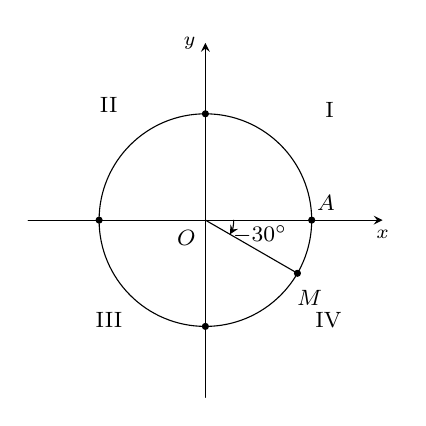
\begin{tikzpicture}[scale=0.9, font=\footnotesize,line join=round, line cap=round, >=stealth];
\draw[->] (-2.5,0) -- (2.5,0) node[below] {\scriptsize $x$};
\draw[->] (0,-2.5) -- (0,2.5) node[left] {\scriptsize $y$};
\draw  (0:0)--(-30:1.5) ;
\draw (0,0) node[below left]{$O$};
\draw  (-30:1.7) node[below]{$M$};
\draw  (45:2.2) node[right]{I} (135:2.3) node[right]{II} (220:2.2) node[right]{III} (315:2) node[right]{IV};
\draw (0:1.5) arc (0:360:1.5);
\draw (-15:0.8) node{$-30^\circ$};
\draw (1.7,0) node[above] {$A$};
\draw[-stealth] (0:.4) arc (0:-30:.4);
\draw[fill=black]  (-1.5,0) circle (1.2pt) (1.5,0) circle (1.2pt)
(0,1.5) circle (1.2pt) (0,-1.5) circle (1.2pt) (-30:1.5) circle (1.2pt);
\end{tikzpicture}
}
}
\end{ex}

\begin{ex}%[Dự án TeX hóa đề cấu trúc mới 2025, Đoàn Hùng]%[1D1N2-4]
Biết $\sin a=-\dfrac{1}{2}$ giá trị của $\sin (\pi -a)$ là
\choice
{$\sin (\pi -a)=\dfrac{1}{2}$}
{\True $\sin (\pi -a)=-\dfrac{1}{2}$}
{$\sin (\pi -a)=\dfrac{\sqrt{3}}{2}$}
{$\sin (\pi -a)=-\dfrac{\sqrt{3}}{2}$}
\loigiai{
Ta có $\sin (\pi -a)=\sin a=-\dfrac{1}{2}$.}
\end{ex}

\begin{ex}%[HK1,Tuy Phong - Bình Thuận, 23-24]%[Đặng Tân Hoài]%[1D1N3-4]
Cho hai góc $a$ và $b$. Khẳng định nào dưới đây đúng?
\choice
{$\sin a+\sin b=2\sin\dfrac{a-b}{2}\cos\dfrac{a+b}{2}$}
{$\sin a+\sin b=2\cos\dfrac{a+b}{2}\cos\dfrac{a-b}{2}$}
{$\sin a+\sin b=-2\sin\dfrac{a-b}{2}\sin\dfrac{a+b}{2}$}
{\True $\sin a+\sin b=2\sin\dfrac{a+b}{2}\cos\dfrac{a-b}{2}$}
\loigiai{
Theo công thức tổng thành tích, ta có $\sin a+\sin b=2\sin\dfrac{a+b}{2}\cos\dfrac{a-b}{2}$.
}
\end{ex}

\begin{ex}%[Dự án 10-11EX-HK1-2324]%[Dao-V- Thuy]%[1D1N4-2]
Tập xác định của hàm số $y=\cot x$ là
\choice
{\True $\mathbb{R} \setminus \{k\pi, \, k\in \mathbb{Z}\}$}
{$\mathbb{R} \setminus \left\{\dfrac{\pi}{2}+k\pi, \, k\in \mathbb{Z}\right\}$}
{$\mathbb{R}$}
{$\mathbb{R} \setminus \{0\}$}
\loigiai
{
Tập xác định của hàm số $y=\cot x$ là $\mathbb{R} \setminus \{k\pi, \, k\in \mathbb{Z}\}$.
}
\end{ex}

\begin{ex}%[HK1 chuyên Hoàng Lê Kha, 2023-2024]%[Trần Chiến, 10-11EX-HK1-23-24]%[1D1N5-1]
Cho số thực $m$ với $|m|\leq 1$. Đồ thị hàm số $y=\cos x$ và đường thẳng $y=m$ được vẽ trên cùng hệ trục tọa độ $Oxy$ như hình bên dưới, trong đó $\alpha$ là góc thuộc $[0;\pi]$ sao cho $\cos\alpha=m$.
% \begin{center}
% \begin{tikzpicture}[scale=0.7, font=\footnotesize, line join=round, line cap=round, >=stealth]
% \draw[->] (-10.5,0) -- (11,0) node[right] {\small $x$};
% \draw[->] (0,-1.8) -- (0,2) node[right] {\small $y$};
% \draw (0,0) circle(1.2pt) node[below right = -0.05 and -0.1] {$O$};
% \draw[color=blue,thick,samples=100,domain=-10.5:10.5] plot(\x,{cos((\x)*180/pi)});
% \draw[dashed] (-3.14,-1)--(-3.14,0) circle(1.2pt) node[below left = 0 and -0.05] {$-\pi$};
% \draw[dashed] (3.14,-1)--(3.14,0) circle(1.2pt) node[below right = 0.05 and -0.05] {$\pi$};
% \draw[fill=black] (-6.283,0) circle(1.2pt) node[below] {$-2\pi$};
% \draw[fill=black] (-9.425,0) circle(1.2pt) node[below] {$-3\pi$};
% \draw[fill=black] (6.283,0) circle(1.2pt) node[below] {$2\pi$};
% \draw[fill=black] (9.425,0) circle(1.2pt) node[below] {$3\pi$};
% \draw[dashed] (-10.5,1)--(10.5,1);
% \draw[dashed] (-10.5,-1)--(10.5,-1);
% \draw[fill=black] (0,-1) circle(1.5pt) node[below left] {$-1$};
% \draw[fill=black] (0,1) circle(1.5pt) node[above left] {$1$};
% \draw[<->] (-3.14,-2)--(3.14,-2) node[midway, below]{$2\pi$};
% \draw[color=red, thick] (-10.5,0.5)--(10.5,0.5);
% \draw[fill=black, dashed] (-1.0472,0.5) circle(1.2pt) -- (-1.0472,0) circle(1.2pt) node[below]{$-\alpha$};
% \draw[fill=black, dashed] (1.0472,0.5) circle(1.2pt) -- (1.0472,0) circle(1.2pt) node[below = 0.07]{$\alpha$};
% \node[right] at (10.4,-0.57) {\color{blue}{$y=\cos x$}};
% \node[right] at (10.4,0.5) {\color{red}{$y=m$}};
% \end{tikzpicture}
% \end{center}
Khi đó, phương trình lượng giác $\cos x=m$ có nghiệm là
\choice
{\True $x=\alpha+k2\pi$ ($k\in\mathbb{Z}$) và $x=-\alpha+k2\pi$ ($k\in\mathbb{Z}$)}
{$x=\alpha+k2\pi$ ($k\in\mathbb{Z}$) và $x=\pi-\alpha+k2\pi$ ($k\in\mathbb{Z}$)}
{$x=\alpha+k\pi$ ($k\in\mathbb{Z}$) và $x=-\alpha+k\pi$ ($k\in\mathbb{Z}$)}
{$x=\alpha+k\pi$ ($k\in\mathbb{Z}$)}
\loigiai{

}
\end{ex}

\TNTF \textit{(4,0 điểm)}
\begin{ex}%[Hoàng Thanh Phương, 24-25 BG K11]%[1D1H3-3]
Cho góc $\alpha$ thỏa mãn $0<\alpha<\dfrac{\pi}{2}$ và $\cos\alpha=\dfrac{3}{4}$. Các khẳng định sau là đúng hay sai?
\choiceTF
{\True $\sin (\pi -\alpha)=\dfrac{\sqrt{7}}{4}$}
{\True $\sin 2\alpha=\dfrac{3\sqrt{7}}{8}$}
{$\sin \dfrac{\alpha}{2}=\dfrac{\sqrt{2}}{8}$}
{$\tan 2\alpha=-3\sqrt{7}$}
\loigiai{
Ta có $0<\alpha<\dfrac{\pi}{2}$ nên $\sin \alpha>0$. \\
Mặt khác, $\cos^2\alpha+\sin^2\alpha=1\Leftrightarrow \sin^2\alpha=\dfrac{7}{16}\Rightarrow\sin\alpha=\dfrac{\sqrt{7}}{4}$.
\begin{itemchoice}
\itemch Ta có $\sin (\pi-\alpha)=\sin \alpha=\dfrac{\sqrt{7}}{4}$.
\itemch Ta có $\sin 2\alpha=2\sin\alpha\cos\alpha=2\cdot \dfrac{\sqrt{7}}{4}\cdot\dfrac{3}{4}=\dfrac{3\sqrt{7}}{8}$.
\itemch Ta có $0<\alpha<\dfrac{\pi}{2}$ nên $0<\dfrac{\alpha}{2}<\dfrac{\pi}{4}$. Vậy $\sin \dfrac{\alpha}{2}>0$. \\
Áp dụng công thức hạ bậc ta có
\[\sin^2\dfrac{\alpha}{2}=\dfrac{1-\cos \alpha}{2}=\dfrac{1}{8}\Rightarrow \sin \dfrac{\alpha}{2}=\dfrac{\sqrt{2}}{4}.\]
\itemch Ta có $\tan \alpha=\dfrac{\sin \alpha}{\cos \alpha}=\dfrac{\sqrt{7}}{3}$.
Vậy $\tan 2\alpha=\dfrac{2\tan \alpha}{1-\tan^2\alpha}=3\sqrt{7}$.
\end{itemchoice}


}
\end{ex}

\begin{ex}%[1-HK1-CT-6-HungVuong-HCM-2324]%[VN-MT-6, Thầy Tú TLH]%[1D1H5-3]
Cho phương trình $3\cos x=m$ (1).
\choiceTF
{\True Khi $m=5$ thì phương trình (1) vô nghiệm}
{\True Có $7$ giá trị nguyên của tham số $m$ để phương trình (1) có nghiệm}
{Khi $m=-3$ thì phương trình (1) có tổng các nghiệm trên khoảng $(0; 4\pi)$ bằng $9\pi$}
{Gọi $T$ (rad) là nghiệm dương nhỏ nhất của phương trình (1) khi $m=-3$. Cho biết kim giờ và kim phút của một đồng hồ lớn có độ dài lần lượt là $17{,}5$ cm và $23{,}5$ cm. Khi kim phút quay được một góc có số đo bằng $T$ (rad) thì kim giờ và kim phút vạch được các cung tròn có tổng độ dài lớn hơn $79$\,cm}
\loigiai{
\begin{itemchoice}
\itemch {\bf Đúng.}\\
Khi $m=5$, phương trình (1) trở thành $3\cos x=5\Leftrightarrow \cos x=\dfrac{5}{3}$.\\
Vì $-1\leq \cos x \leq 1$, $\forall x \in \mathbb{R}$ nên phương trình $\cos x=\dfrac{5}{3}$ vô nghiệm.
\itemch {\bf Đúng.}\\
Ta có $-1\leq \cos x \leq 1$, $\forall x \in \mathbb{R}$ suy ra $-3\leq 3\cos x \leq 3$.\\
Để phương trình có nghiệm thì $-3\leq m \leq 3$.\\
Mà $m$ là số nguyên nên $m \in \{-3;-2;-1;0;1;2;3\}$.\\
Vậy có $7$ giá trị nguyên $m$ thoả mãn.
\itemch {\bf Sai.}\\
Khi $m=-3$, phương trình (1) trở thành
\[3\cos x=-3\Leftrightarrow \cos x=-1\Leftrightarrow x=\pi+k2\pi,\,k\in \mathbb {Z}.\]
Vì $x\in (0;4\pi)$ nên $x=\pi$ hoặc $x=3\pi$.\\
Vậy tổng các nghiệm trên bằng $4\pi$.
\itemch {\bf Sai.}\\
Khi $m=-3$, phương trình $\cos x=-1$ có nghiệm dương nhỏ nhất bằng $\pi$.\\
Theo đề bài ta có kim phút quay được một góc có số đo là $\pi$ (rad).\\
Khi đó kim giờ quay được góc có số đo là \[\dfrac{2\pi}{12}\cdot \dfrac{\pi}{2\pi}=\dfrac{\pi}{12}.\]
Suy ra tổng độ dài các cung tròn mà kim phút và kim giờ quay được là
\[\ell=\pi \cdot 23{,}5+\dfrac {\pi}{12}\cdot 17{,}5\approx 78{,}4\,\text{(cm)}.\]
\end{itemchoice}
}
\end{ex}

\TNSA \textit{(2,0 điểm)}
\begin{ex}%[Cánh diều]%[Đỗ Vũ Minh Thắng, 24-25 BG 10 11]%[1D1V3-2]
Một sợi cáp $R$ được gắn vào một cột thẳng đứng ở vị trí cách mặt đất $14$ m. Một sợi cáp $S$ khác cũng được gắn vào cột đó ở vị trí cách mặt đất $12$ m. Biết rằng hai sợi cáp trên cùng được gắn với mặt đất tại một vị trí cách chân cột $15$ m.
\begin{center}
\begin{tikzpicture}[>=stealth,line join=round,line cap=round,font=\footnotesize,scale=.7]
\path
(0,0) coordinate (H)node[below]{$H$}
(-0.2,0) coordinate (H1)
(7.5,0) coordinate (O)node[below]{$O$}
(0,7) coordinate (A)node[above]{$A$}
(0,5) coordinate (B)node[above left, shift={(160:3pt)}]{$B$}
(2,1.7) coordinate (I)
(2.2,1.7) coordinate (I1)
($(B)-(H)+(I)$) coordinate (J)
(2.07,6.6)coordinate (J1)
($(A)-(H)+(I)$) coordinate (K)
($(K)-(I)+(I1)$) coordinate (K1)
($(A)-(B)+(J1)$) coordinate (K2)
($(A)-(H)+(H1)$) coordinate (A1)
;
\fill[blue!45]
(A)--(A1)--(H1)--(H)--cycle
(I)--(I1)--(K1)--(K)--cycle
;
\draw[<->]
(-.85,0)--(-.85,5) node[fill=white,inner sep=2pt,midway]{$12$ m}
;
\draw[<->]
(-1.7,0)--(-1.7,7) node[fill=white,inner sep=2pt,midway]{$14$ m}
;
\draw[dashed]
(-1.7,0)--(H1)
(-.85,5)--(-.2,5)
(-1.7,7)--(A1)
;
\draw[red]
(A)--(O)node[pos=.5,above,black]{$R$}
(B)--(O)node[pos=.45,below,black]{$S$}
;
\draw[<->]
(-0.07,-0.05)--(O)node[pos=.5,below]{$15$ m}
;
\draw
(H)--(H1)--(A1)--(A)--cycle--(I)--(K)--(K1)--(I1)--(I)
(B)--(J1)
(A)--(K2)
(O) pic[draw,angle radius = 25] {angle = A--O--H} node[shift={(160:29pt)}]{$\beta$}
(O) pic[draw,angle radius = 40] {angle = A--O--B} node[shift={(142:45pt)}]{$\alpha$}
(O) pic[draw,angle radius = 41] {angle = A--O--B}
;
\end{tikzpicture}
\end{center}
Tìm góc $\alpha$ (làm tròn kết quả đến hàng đơn vị theo đơn vị độ).
\shortans{4}
\loigiai{
Ta có $\tan\widehat{AOH}=\dfrac{AH}{OH}=\dfrac{14}{15}$, $\tan\widehat{BOH}=\dfrac{BH}{OH}=\dfrac{12}{15}$. Suy ra:\\ $\tan\alpha=\tan\widehat{AOB}=\tan\left(\widehat{AOH}-\widehat{BOH}\right)=\dfrac{\ tan\widehat{AOH}-\tan\widehat{BOH}}{1+\tan\widehat{AOH}\cdot\tan\widehat{BOH}}=\dfrac{\frac{14}{15}-\frac{12}{15}}{1+\frac{14}{15}\cdot\frac{12}{15}}=\dfrac{10}{131}$.\\
$\tan\alpha=\dfrac{10}{131}\Rightarrow\alpha\approx 4^\circ$.
}
\end{ex}

\begin{ex}%[1D1V5-5]
Phương trình $\cos x+\cos 2x=0$ có tất cả bao nhiêu nghiệm thuộc đoạn $[-\pi;\pi]$?
\shortans[]{$4$}
\loigiai{{\allowdisplaybreaks
\begin{eqnarray*}
& & \cos x+\cos 2x=0
\Leftrightarrow 2\cos^2x+\cos x-1=0\\
&\Leftrightarrow&
\hoac{&\cos x=-1\\&\cos x=\dfrac{1}{2}}
\Leftrightarrow \hoac{&x=\pi+k2\pi \\&x=\pm\dfrac{\pi}{3}+k2\pi},\,(k\in\mathbb{Z}).
\end{eqnarray*}
Trên đoạn $[-\pi;\pi]$
\begin{itemize}
\item Họ nghiệm $x=\pi+k2\pi$ có hai nghiệm $x=\pm \pi$.
\item Họ nghiệm $x=\dfrac{\pi}{3}+k2\pi$ có một nghiệm $x=\dfrac{\pi}{3}$.
\item Họ nghiệm $x=-\dfrac{\pi}{3}+k2\pi$ có một nghiệm $x=-\dfrac{\pi}{3}$.
\end{itemize}
}
Vậy phương trình có tất cả $4$ nghiệm trên đoạn $[-\pi;\pi]$.
}
\end{ex}
\TL \textit{(1,0 điểm)}
\begin{ex}%[Mức H, KNTT]%[BG Toán 11 CT2025, Quan Ón]%[1D1H5-3]
Giải các phương trình sau
\begin{listEX}[2]
\item $\sin 2x  = \sin (60^{\circ} - 3x)$;
\item $\cos 2 x=\cos \left(45^{\circ}-x\right)$.
\end{listEX}
\loigiai{
\begin{enumerate}
\item $\sin2x=\sin(60^{\circ}-3x)\Leftrightarrow\hoac{&2x=60^\circ-3x+k360^\circ\\&2x=3x+120^\circ+k360^\circ}\Leftrightarrow\hoac{&x=12^\circ+k72^\circ\\&x=-120^\circ-k360^\circ},\,(k \in \mathbb{Z})$.
\item $\cos2x=\cos\left(45^{\circ}-x\right)  \Leftrightarrow\hoac{&2 x=45^{\circ}-x+k 360^{\circ}\\&2x=-\left(45^{\circ}-x\right)+k 360^{\circ}} \Leftrightarrow\hoac{&3x=45^{\circ}+k360^{\circ}\\&x=-45^{\circ}+k360^{\circ}}\\\Leftrightarrow \hoac{&x=15^{\circ}+k 120^{\circ} \\&x=-45^{\circ}+k 360^{\circ}},\,(k \in \mathbb{Z})$.
\end{enumerate}
}

\end{ex}
\dongcham{10}